\chapter{Programmbeschreibung}\label{ch:programmbeschreibung}

\section{Entwurf}\label{sec:entwurf}
In der Planung wurde das Strategie-Entwurfsmuster als
\pagebreak

\section{UML-Diagramme}\label{sec:uml}

\noindent%
\begin{minipage}{\linewidth}% to keep image and caption on one page
    \makebox[\linewidth]{%        to center the image
        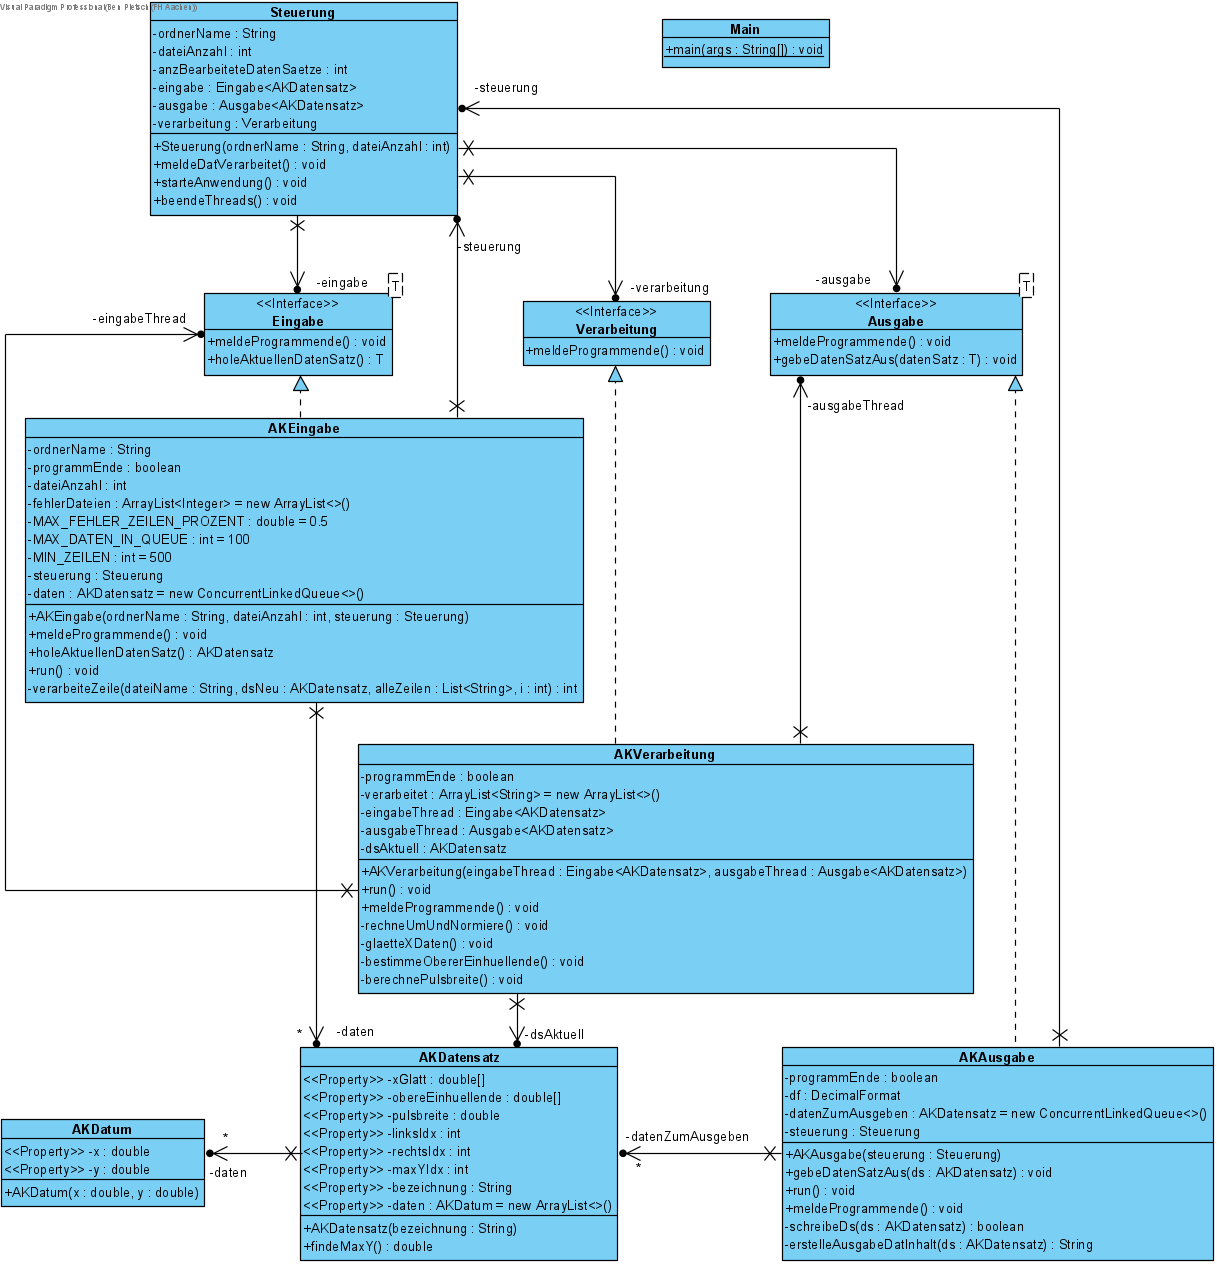
\includegraphics[keepaspectratio=true,scale=0.7]{images/ClassDiagram1}}
    \captionof{figure}{Klassendiagramm.}\label{fig:klassen-dia}
\end{minipage}

\noindent%
\begin{minipage}{\linewidth}% to keep image and caption on one page
    \makebox[\linewidth]{%        to center the image
        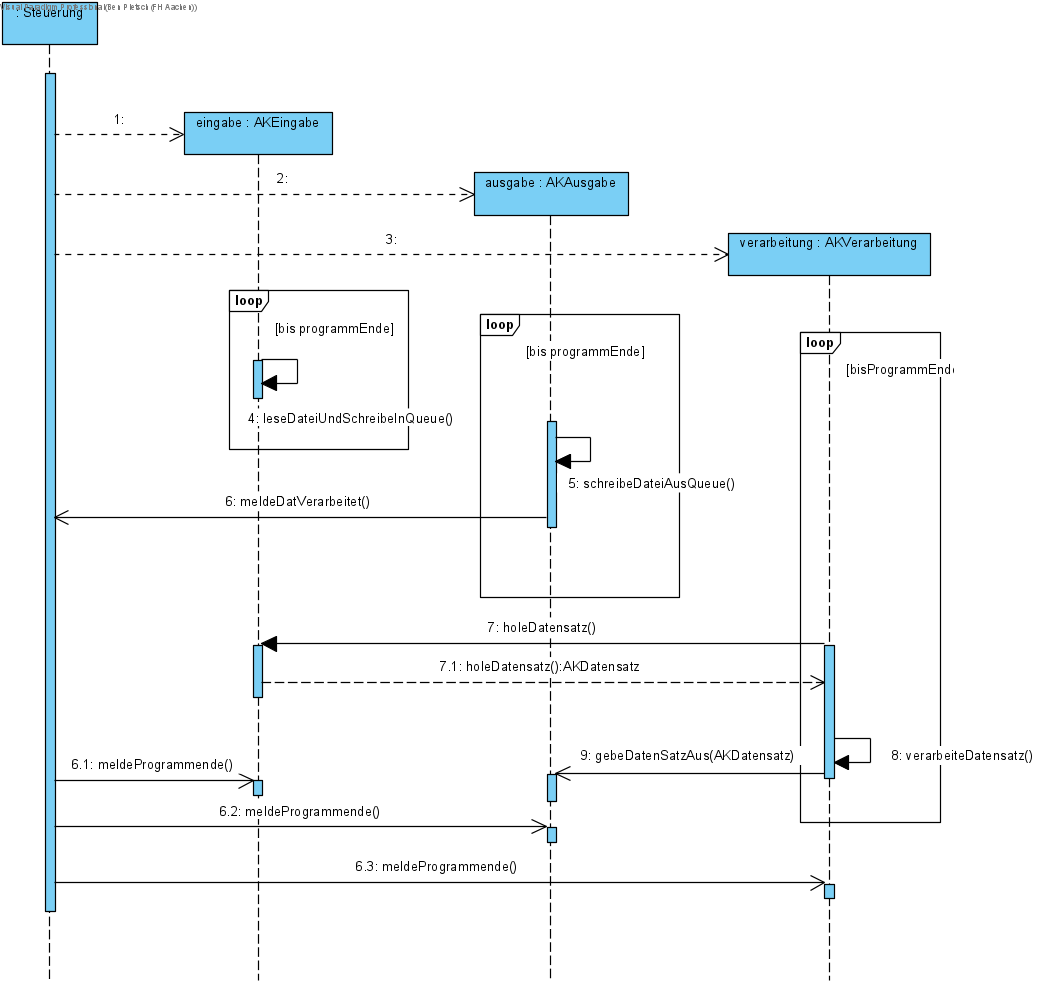
\includegraphics[keepaspectratio=true,scale=0.8]{images/sequenz}}
    \captionof{figure}{Sequenzdiagramm.}\label{fig:sequenz}
\end{minipage}


\section{Struktogramme}\label{sec:strukto}

\noindent%
\begin{minipage}{\linewidth}% to keep image and caption on one page
    \makebox[\linewidth]{%        to center the image
        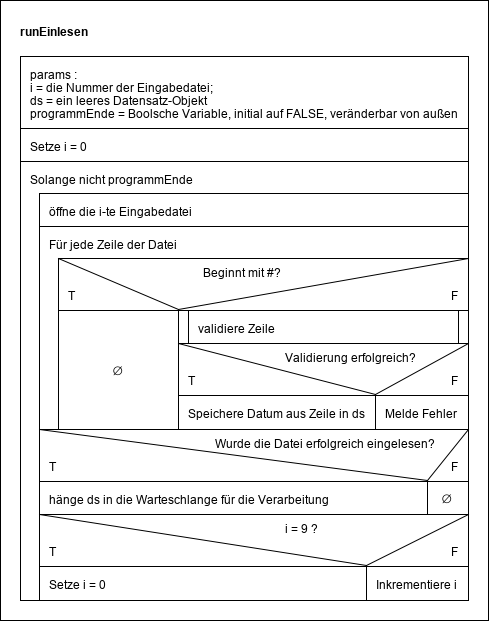
\includegraphics[keepaspectratio=true,scale=0.4]{images/runEinlesen}}
    \captionof{figure}{Vorgehen beim Einlesen der Textdateien.}\label{fig:run-einlesen}
\end{minipage}

\noindent%
\begin{minipage}{\linewidth}% to keep image and caption on one page
    \makebox[\linewidth]{%        to center the image
        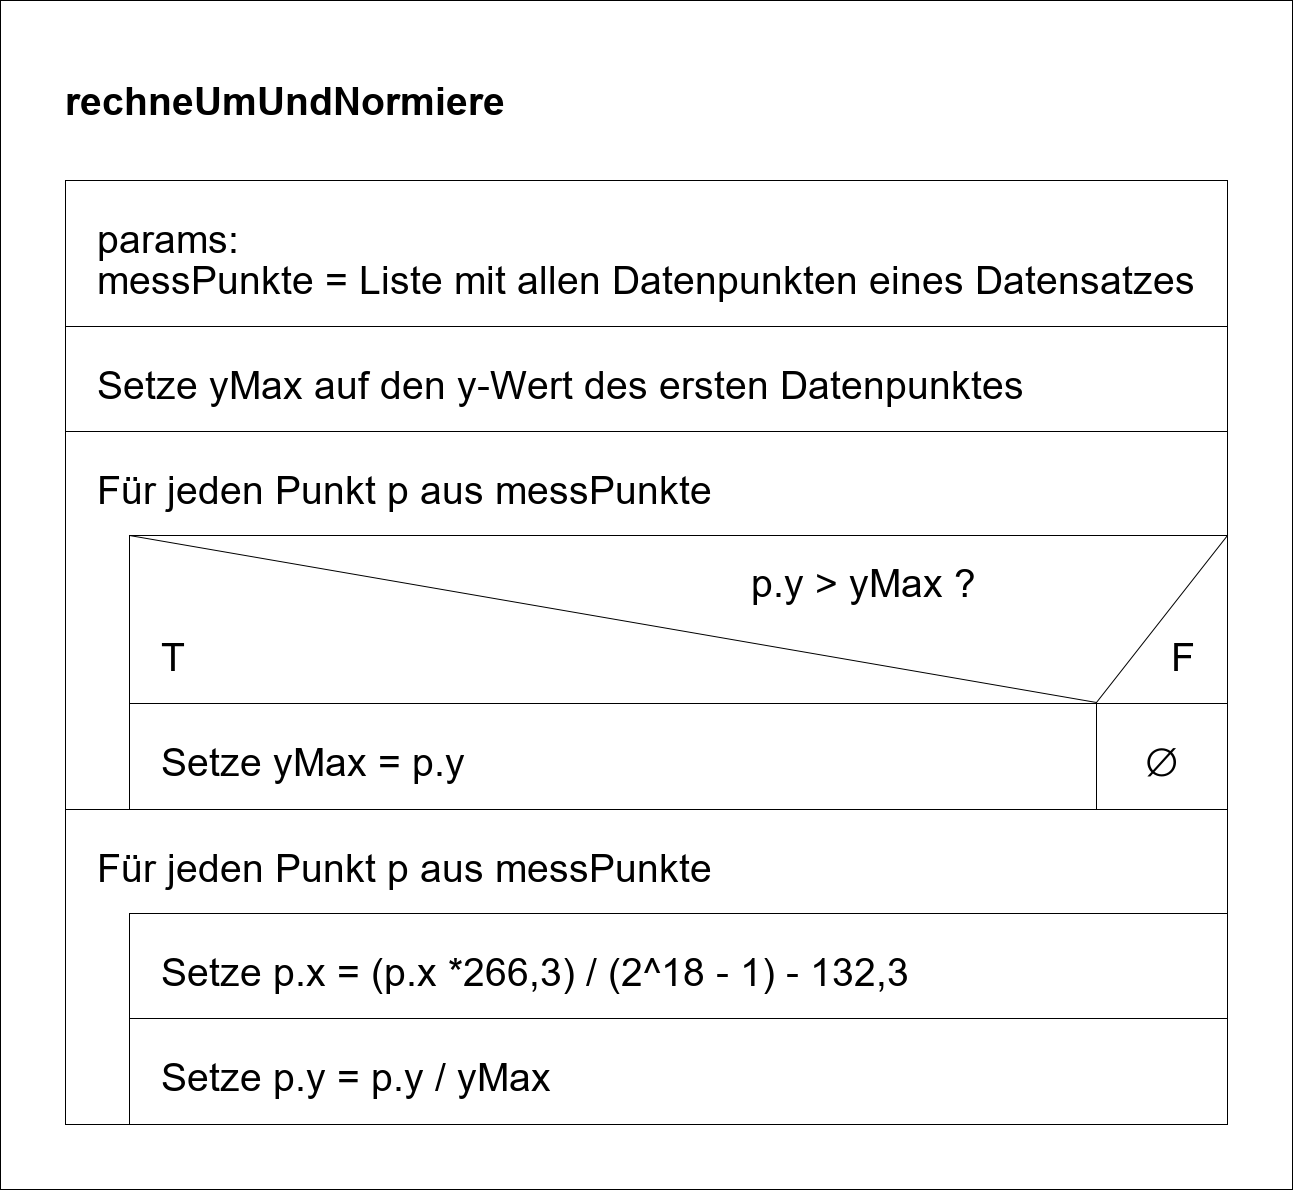
\includegraphics[keepaspectratio=true,scale=0.3]{images/rechneUmUndNormiere}}
    \captionof{figure}{Erster Schritt aus der Verarbeitung, siehe Abschnitt~\ref{subsec:umrechnung-und-normierung}.}\label{fig:umrechnung-normierung}
\end{minipage}


\noindent%
\begin{minipage}{\linewidth}% to keep image and caption on one page
    \makebox[\linewidth]{%        to center the image
        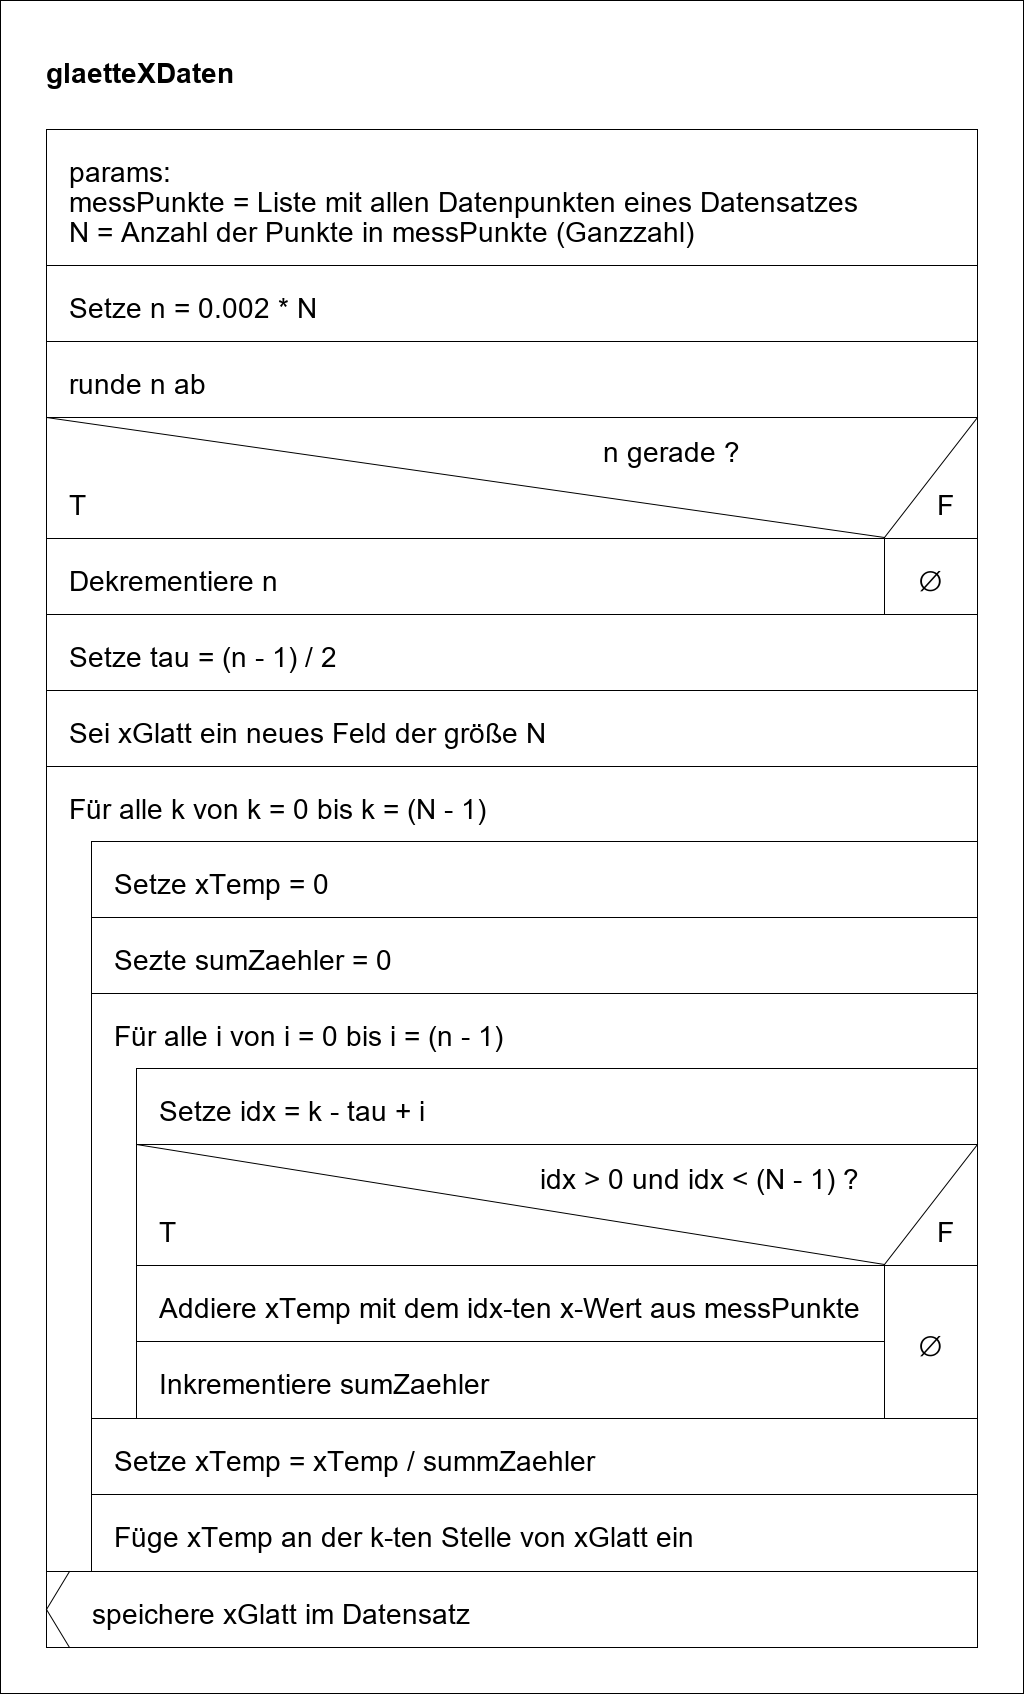
\includegraphics[keepaspectratio=true,scale=0.35]{images/glaetteXDaten}}
    \captionof{figure}{Zweiter Schritt der Verarbeitung, siehe Abschnitt~\ref{subsec:glaettung}.}\label{fig:glaettung-fig}
\end{minipage}

\noindent%
\begin{minipage}{\linewidth}% to keep image and caption on one page
    \makebox[\linewidth]{%        to center the image
        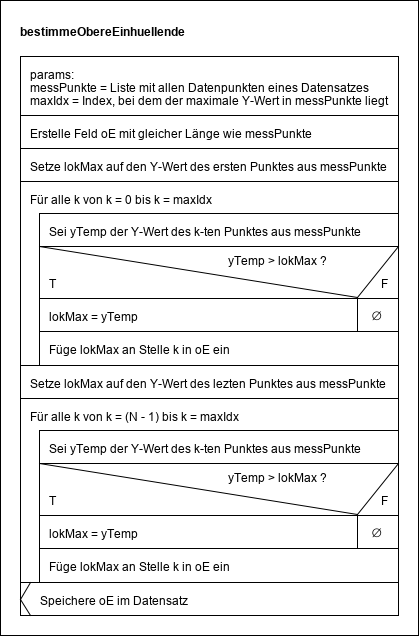
\includegraphics[keepaspectratio=true,scale=0.35]{images/bestimmeObereEinhuellende}}
    \captionof{figure}{Dritter Schritt der Verarbeitung, siehe Abschnitt~\ref{subsec:ober-einh}.}\label{fig:obere-ein-strukto}
\end{minipage}

\noindent%
\begin{minipage}{\linewidth}% to keep image and caption on one page
    \makebox[\linewidth]{%        to center the image
        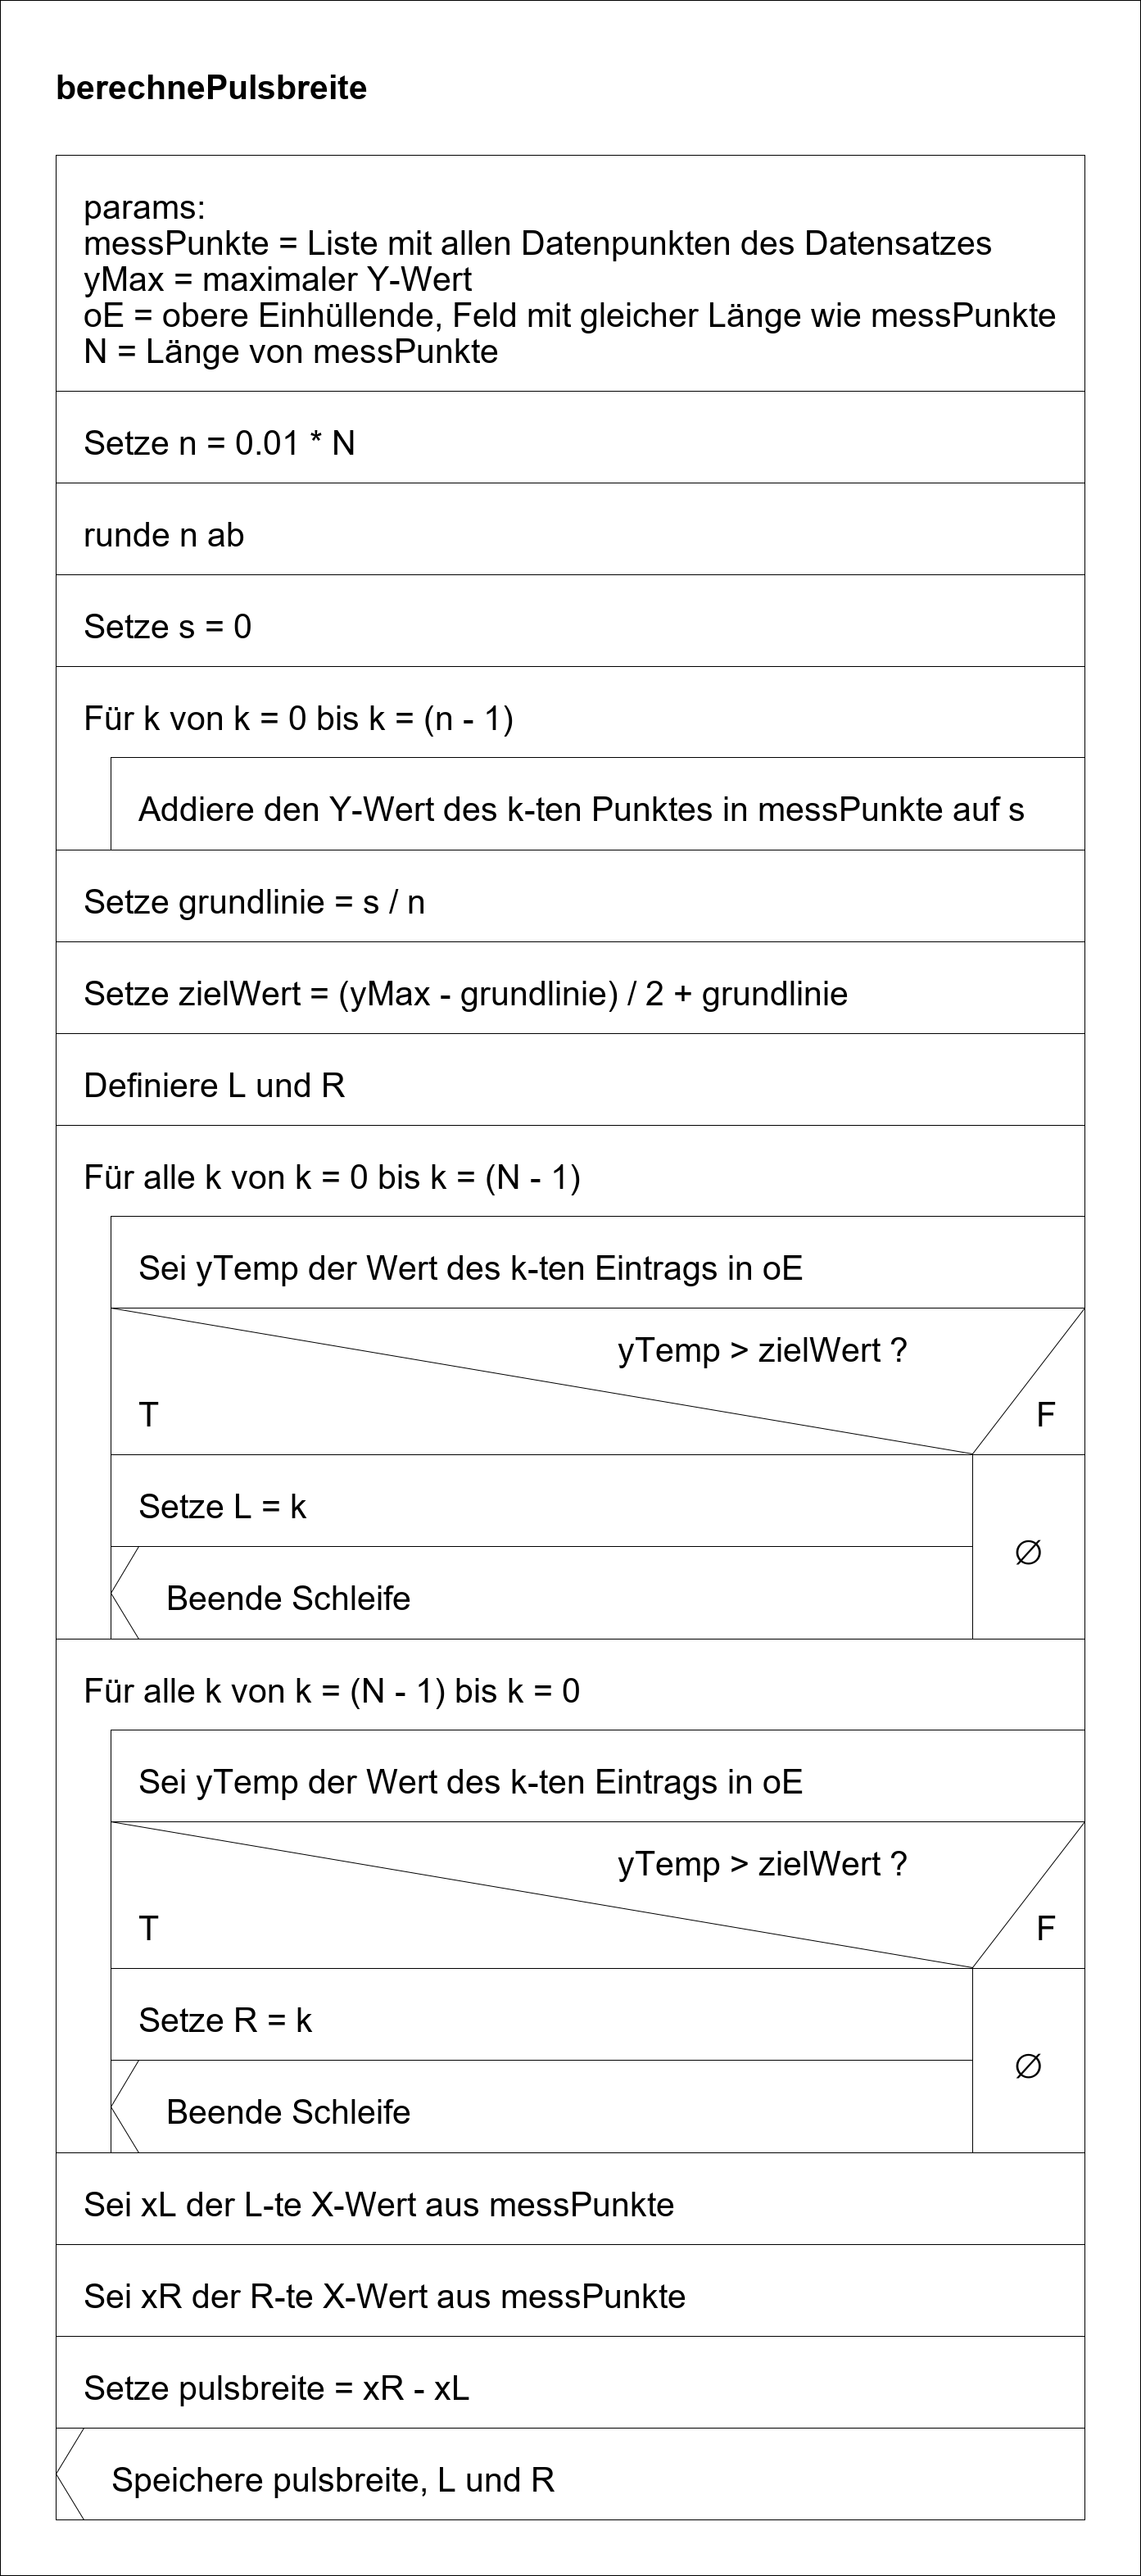
\includegraphics[keepaspectratio=true,scale=0.18]{images/berechnePulsbreite}}
    \captionof{figure}{Vierter Schritt der Verarbeitung, siehe Abschnitt~\ref{subsec:pulsbreite}.}\label{fig:puls-strukto}
\end{minipage}



\section{Entwicklungsdokumentation}\label{sec:entwicklerdokumentation}
Im Abgabe-Ordner befindet sich ein Verzeichnis mit dem Namen \glqq JavaDoc\grqq{}.
Mit einem Doppelklick auf die darin enthaltene Datei \glqq index.html\grqq{} öffnet sich die Dokumentation im Web-Browser.